\documentclass{standalone}
\usepackage{tikz}
\usetikzlibrary{patterns, positioning}


\begin{document}
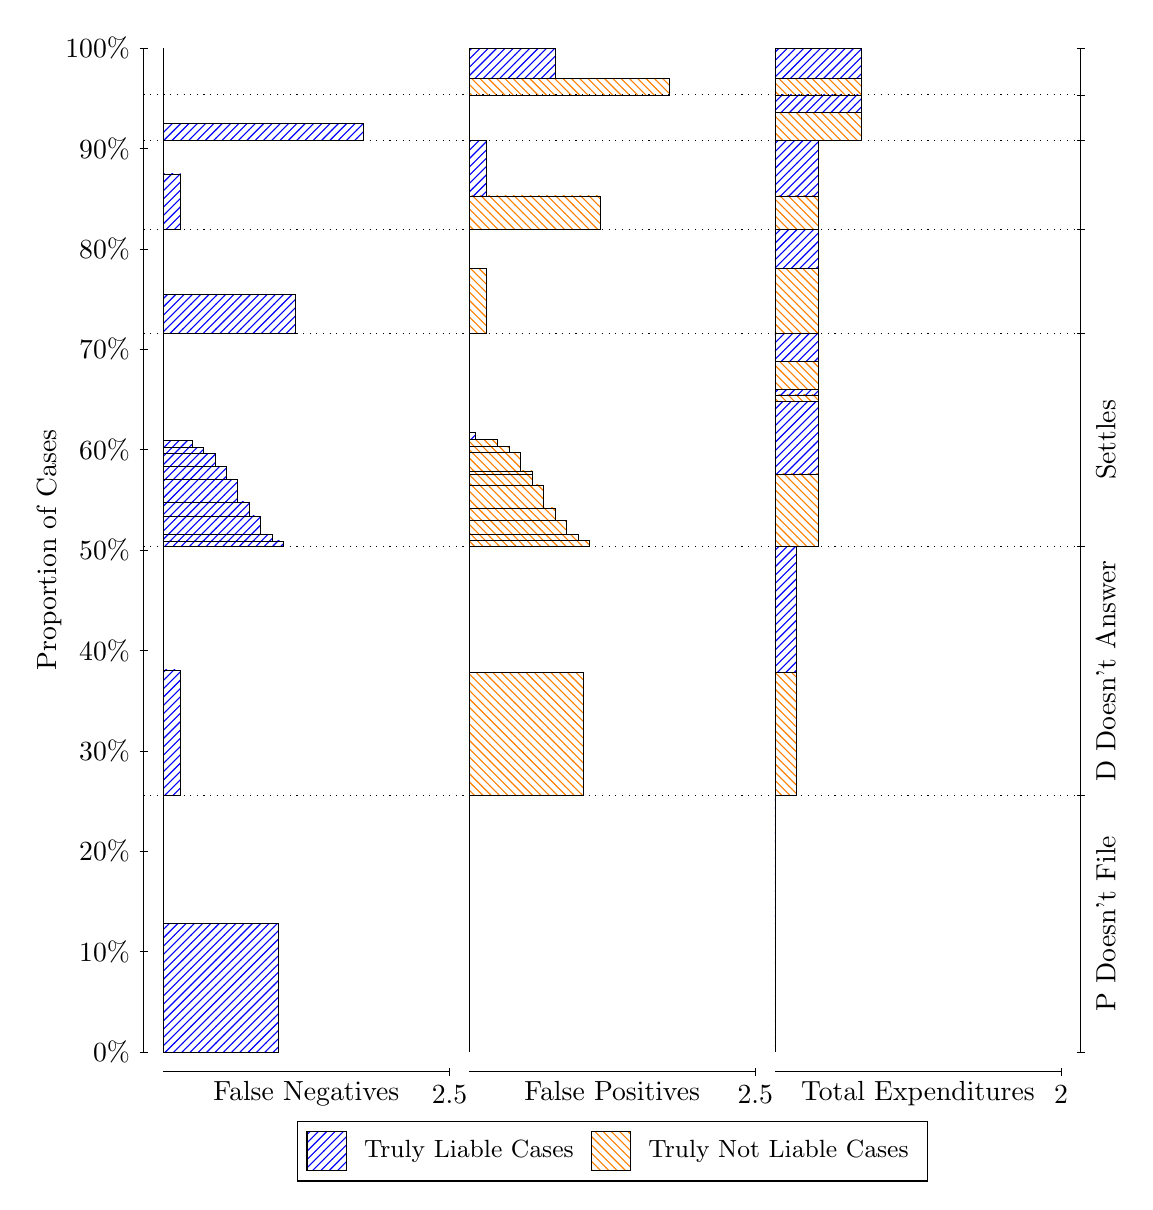
\begin{tikzpicture}
\draw[black, very thin] (1.5,1.75) -- (1.5,14.5);
\node[rotate=90, text=black, anchor=center] at (0.3, 8.125) {Proportion of Cases};
\draw[black, very thin] (1.45,1.75) -- (1.55,1.75);
\node[text=black, anchor=east] at (1.45, 1.75) {0\%};
\draw[black, very thin] (1.45,3.025) -- (1.55,3.025);
\node[text=black, anchor=east] at (1.45, 3.025) {10\%};
\draw[black, very thin] (1.45,4.3) -- (1.55,4.3);
\node[text=black, anchor=east] at (1.45, 4.3) {20\%};
\draw[black, very thin] (1.45,5.575) -- (1.55,5.575);
\node[text=black, anchor=east] at (1.45, 5.575) {30\%};
\draw[black, very thin] (1.45,6.85) -- (1.55,6.85);
\node[text=black, anchor=east] at (1.45, 6.85) {40\%};
\draw[black, very thin] (1.45,8.125) -- (1.55,8.125);
\node[text=black, anchor=east] at (1.45, 8.125) {50\%};
\draw[black, very thin] (1.45,9.4) -- (1.55,9.4);
\node[text=black, anchor=east] at (1.45, 9.4) {60\%};
\draw[black, very thin] (1.45,10.675) -- (1.55,10.675);
\node[text=black, anchor=east] at (1.45, 10.675) {70\%};
\draw[black, very thin] (1.45,11.95) -- (1.55,11.95);
\node[text=black, anchor=east] at (1.45, 11.95) {80\%};
\draw[black, very thin] (1.45,13.225) -- (1.55,13.225);
\node[text=black, anchor=east] at (1.45, 13.225) {90\%};
\draw[black, very thin] (1.45,14.5) -- (1.55,14.5);
\node[text=black, anchor=east] at (1.45, 14.5) {100\%};

\draw[black, very thin] (13.4,1.75) -- (13.4,14.5);
\draw[black, very thin] (13.35,1.75) -- (13.45,1.75);
\node[anchor=west] at (13.35, 1.75) {};
\draw[black, very thin] (13.35,5.0064) -- (13.45,5.0064);
\node[anchor=west] at (13.35, 5.0064) {};
\draw[black, very thin] (13.35,8.1684) -- (13.45,8.1684);
\node[anchor=west] at (13.35, 8.1684) {};
\draw[black, very thin] (13.35,10.878) -- (13.45,10.878);
\node[anchor=west] at (13.35, 10.878) {};
\draw[black, very thin] (13.35,12.2) -- (13.45,12.2);
\node[anchor=west] at (13.35, 12.2) {};
\draw[black, very thin] (13.35,13.324) -- (13.45,13.324);
\node[anchor=west] at (13.35, 13.324) {};
\draw[black, very thin] (13.35,13.905) -- (13.45,13.905);
\node[anchor=west] at (13.35, 13.905) {};
\draw[black, very thin] (13.35,14.5) -- (13.45,14.5);
\node[anchor=west] at (13.35, 14.5) {};

\draw[black, very thin, pattern color=blue, pattern=north east lines] (1.75,1.75) rectangle (3.2033,3.3782);
\draw[black, very thin, pattern color=orange, pattern=north west lines] (1.75,3.3782) rectangle (1.75,5.0064);
\draw[black, very thin, pattern color=blue, pattern=north east lines] (1.75,5.0064) rectangle (1.968,6.6036);
\draw[black, very thin, pattern color=orange, pattern=north west lines] (1.75,6.6036) rectangle (1.75,8.1684);
\draw[black, very thin, pattern color=blue, pattern=north east lines] (1.75,8.1684) rectangle (3.276,8.2394);
\draw[black, very thin, pattern color=blue, pattern=north east lines] (1.75,8.2394) rectangle (3.1307,8.3234);
\draw[black, very thin, pattern color=blue, pattern=north east lines] (1.75,8.3234) rectangle (2.9853,8.5595);
\draw[black, very thin, pattern color=blue, pattern=north east lines] (1.75,8.5595) rectangle (2.84,8.7368);
\draw[black, very thin, pattern color=blue, pattern=north east lines] (1.75,8.7368) rectangle (2.6947,9.0254);
\draw[black, very thin, pattern color=blue, pattern=north east lines] (1.75,9.0254) rectangle (2.5493,9.188);
\draw[black, very thin, pattern color=blue, pattern=north east lines] (1.75,9.188) rectangle (2.404,9.3544);
\draw[black, very thin, pattern color=blue, pattern=north east lines] (1.75,9.3544) rectangle (2.2587,9.4246);
\draw[black, very thin, pattern color=blue, pattern=north east lines] (1.75,9.4246) rectangle (2.1133,9.5204);
\draw[black, very thin, pattern color=orange, pattern=north west lines] (1.75,9.5204) rectangle (1.75,10.878);
\draw[black, very thin, pattern color=blue, pattern=north east lines] (1.75,10.878) rectangle (3.4213,11.372);
\draw[black, very thin, pattern color=orange, pattern=north west lines] (1.75,11.372) rectangle (1.75,12.2);
\draw[black, very thin, pattern color=blue, pattern=north east lines] (1.75,12.2) rectangle (1.968,12.901);
\draw[black, very thin, pattern color=orange, pattern=north west lines] (1.75,12.901) rectangle (1.75,13.324);
\draw[black, very thin, pattern color=blue, pattern=north east lines] (1.75,13.324) rectangle (4.2933,13.543);
\draw[black, very thin, pattern color=orange, pattern=north west lines] (1.75,13.543) rectangle (1.75,13.905);
\draw[black, very thin, pattern color=orange, pattern=north west lines] (1.75,13.905) rectangle (1.75,14.117);
\draw[black, very thin, pattern color=blue, pattern=north east lines] (1.75,14.117) rectangle (1.75,14.5);
\draw[black, very thin, pattern color=orange, pattern=north west lines] (5.6333,1.75) rectangle (5.6333,3.3782);
\draw[black, very thin, pattern color=blue, pattern=north east lines] (5.6333,3.3782) rectangle (5.6333,5.0064);
\draw[black, very thin, pattern color=orange, pattern=north west lines] (5.6333,5.0064) rectangle (7.0867,6.5712);
\draw[black, very thin, pattern color=blue, pattern=north east lines] (5.6333,6.5712) rectangle (5.6333,8.1684);
\draw[black, very thin, pattern color=orange, pattern=north west lines] (5.6333,8.1684) rectangle (7.1593,8.2454);
\draw[black, very thin, pattern color=orange, pattern=north west lines] (5.6333,8.2454) rectangle (7.014,8.3229);
\draw[black, very thin, pattern color=orange, pattern=north west lines] (5.6333,8.3229) rectangle (6.8687,8.4983);
\draw[black, very thin, pattern color=orange, pattern=north west lines] (5.6333,8.4983) rectangle (6.7233,8.6598);
\draw[black, very thin, pattern color=orange, pattern=north west lines] (5.6333,8.6598) rectangle (6.578,8.9507);
\draw[black, very thin, pattern color=orange, pattern=north west lines] (5.6333,8.9507) rectangle (6.4327,9.0914);
\draw[black, very thin, pattern color=orange, pattern=north west lines] (5.6333,9.0914) rectangle (6.4327,9.1297);
\draw[black, very thin, pattern color=orange, pattern=north west lines] (5.6333,9.1297) rectangle (6.2873,9.3625);
\draw[black, very thin, pattern color=orange, pattern=north west lines] (5.6333,9.3625) rectangle (6.142,9.4442);
\draw[black, very thin, pattern color=orange, pattern=north west lines] (5.6333,9.4442) rectangle (5.9967,9.5262);
\draw[black, very thin, pattern color=blue, pattern=north east lines] (5.6333,9.5262) rectangle (5.706,9.6219);
\draw[black, very thin, pattern color=blue, pattern=north east lines] (5.6333,9.6219) rectangle (5.6333,10.878);
\draw[black, very thin, pattern color=orange, pattern=north west lines] (5.6333,10.878) rectangle (5.8513,11.706);
\draw[black, very thin, pattern color=blue, pattern=north east lines] (5.6333,11.706) rectangle (5.6333,12.2);
\draw[black, very thin, pattern color=orange, pattern=north west lines] (5.6333,12.2) rectangle (7.3047,12.622);
\draw[black, very thin, pattern color=blue, pattern=north east lines] (5.6333,12.622) rectangle (5.8513,13.324);
\draw[black, very thin, pattern color=orange, pattern=north west lines] (5.6333,13.324) rectangle (5.6333,13.686);
\draw[black, very thin, pattern color=blue, pattern=north east lines] (5.6333,13.686) rectangle (5.6333,13.905);
\draw[black, very thin, pattern color=orange, pattern=north west lines] (5.6333,13.905) rectangle (8.1767,14.117);
\draw[black, very thin, pattern color=blue, pattern=north east lines] (5.6333,14.117) rectangle (6.7233,14.5);
\draw[black, very thin, pattern color=orange, pattern=north west lines] (9.5167,1.75) rectangle (9.5167,3.3782);
\draw[black, very thin, pattern color=blue, pattern=north east lines] (9.5167,3.3782) rectangle (9.5167,5.0064);
\draw[black, very thin, pattern color=orange, pattern=north west lines] (9.5167,5.0064) rectangle (9.7892,6.5712);
\draw[black, very thin, pattern color=blue, pattern=north east lines] (9.5167,6.5712) rectangle (9.7892,8.1684);
\draw[black, very thin, pattern color=orange, pattern=north west lines] (9.5167,8.1684) rectangle (10.062,9.0914);
\draw[black, very thin, pattern color=blue, pattern=north east lines] (9.5167,9.0914) rectangle (10.062,10.014);
\draw[black, very thin, pattern color=orange, pattern=north west lines] (9.5167,10.014) rectangle (10.062,10.096);
\draw[black, very thin, pattern color=blue, pattern=north east lines] (9.5167,10.096) rectangle (10.062,10.167);
\draw[black, very thin, pattern color=orange, pattern=north west lines] (9.5167,10.167) rectangle (10.062,10.52);
\draw[black, very thin, pattern color=blue, pattern=north east lines] (9.5167,10.52) rectangle (10.062,10.878);
\draw[black, very thin, pattern color=orange, pattern=north west lines] (9.5167,10.878) rectangle (10.062,11.706);
\draw[black, very thin, pattern color=blue, pattern=north east lines] (9.5167,11.706) rectangle (10.062,12.2);
\draw[black, very thin, pattern color=orange, pattern=north west lines] (9.5167,12.2) rectangle (10.062,12.622);
\draw[black, very thin, pattern color=blue, pattern=north east lines] (9.5167,12.622) rectangle (10.062,13.324);
\draw[black, very thin, pattern color=orange, pattern=north west lines] (9.5167,13.324) rectangle (10.607,13.686);
\draw[black, very thin, pattern color=blue, pattern=north east lines] (9.5167,13.686) rectangle (10.607,13.905);
\draw[black, very thin, pattern color=orange, pattern=north west lines] (9.5167,13.905) rectangle (10.607,14.117);
\draw[black, very thin, pattern color=blue, pattern=north east lines] (9.5167,14.117) rectangle (10.607,14.5);
\draw[black, dotted] (1.5,5.0064) -- (13.4,5.0064);
\draw[black, dotted] (1.5,8.1684) -- (13.4,8.1684);
\draw[black, dotted] (1.5,10.878) -- (13.4,10.878);
\draw[black, dotted] (1.5,12.2) -- (13.4,12.2);
\draw[black, dotted] (1.5,13.324) -- (13.4,13.324);
\draw[black, dotted] (1.5,13.905) -- (13.4,13.905);
\draw[black, very thin] (1.75,1.5) -- (5.3833,1.5);
\node[text=black, anchor=north] at (3.5667, 1.5) {False Negatives};
\draw[black, very thin] (5.3833,1.45) -- (5.3833,1.55);
\node[text=black, anchor=north] at (5.3833, 1.45) {2.5};

\draw[black, very thin] (5.6333,1.5) -- (9.2667,1.5);
\node[text=black, anchor=north] at (7.45, 1.5) {False Positives};
\draw[black, very thin] (9.2667,1.45) -- (9.2667,1.55);
\node[text=black, anchor=north] at (9.2667, 1.45) {2.5};

\draw[black, very thin] (9.5167,1.5) -- (13.15,1.5);
\node[text=black, anchor=north] at (11.333, 1.5) {Total Expenditures};
\draw[black, very thin] (13.15,1.45) -- (13.15,1.55);
\node[text=black, anchor=north] at (13.15, 1.45) {2};

\node[text=black, centered, rotate=90] at (13.72, 3.3782) {P Doesn't File};
\node[text=black, centered, rotate=90] at (13.72, 6.5874) {D Doesn't Answer};
\node[text=black, centered, rotate=90] at (13.72, 9.5233) {Settles};





\draw (7.449999999999999,1.5) node[draw=none] (baseCoordinate) {};
\begin{scope}[align=center]
        \matrix[scale=0.5, draw=black, below=0.5cm of baseCoordinate, nodes={draw}, column sep=0.1cm]{
            \node[rectangle, draw, minimum width=0.5cm, minimum height=0.5cm, pattern color=blue, pattern=north east lines] {}; &
            \node[draw=none, font=\small, text=black] (B) {Truly Liable Cases}; &
            \node[rectangle, draw, minimum width=0.5cm, minimum height=0.5cm, pattern color=orange, pattern=north west lines] {}; &
            \node[draw=none, font=\small, text=black] (B) {Truly Not Liable Cases}; \\
            };
\end{scope}

\end{tikzpicture}
\end{document}